\chapter{Talk}

\section{Recording}
So what I’m gonna do now is introduce the key ideas that are arranged into like the foundation or something of this thesis that is a theoretical background and then I’m going to describe how we brought these things together in the actual model, and how the model functions and the details of the model, and then I’m going to talk about the results That we got in the models in particular around these key questions of ownership distribution and urban productivity.

I’m trying to think how to like financial in order we’re gonna talk about what financial is specifically and how it is created in. It is done accomplished in the housing market like the specifics of what financial looks like in the housing market. That’s a good face.
And then we’ll go into classical economics to borrow this theory of urban rents, which illuminates not urban, but you know rent to look at rent theory, which illuminates the value, or how spatial how distance how spatial relationships are translated into value in ways, like which make the relationship which make a key relationship between space and economics because economics is about money and productivity and space is something where when you add transportation cost in you have it you have this urban rents give you this connection between how far things are away and how and how much it costs, so so we’ll get into that because that makes this key connection rents the key link Sent this in a few different ways, but rents are the key link between spatial between how far things are away from the centre and the economic questions about productivity that we’re gonna talk about then we’re gonna talk about space which brings in urban theory because there’s a I forget what you talk about in space I never noticed space chapter but space chapter is about about takes up urban rents and develops them through urban theory, and ways that are useful because it is relevant already so we’re talking about how urban rents were taken developed in further in urban theory and then we’re gonna go back into But you already talked about in you talked about marginal marginal that’s in the wrench chapter
Just wanna put in the right order that you have it OK so before you say, bring the urban theory and you would say you would say then we’re gonna talk about more commonly used economic models to for productivity, which are important, so rents gonna make the connection with the spatial and but these are our models of productivity that are relevant because we’re again I think the key thing you’re gonna keep hitting because it’s a verbal presentation is we’re making this connection between space and economics And so we need these things so the economic things kind of when you move out of the rent they lose track of they they leave behind the spatial and we’re gonna but we’re gonna use some of these elements from marginal so we’ll introduce that then we’re gonna go back into the spatial and see how urban rents were developed into urban theory, which is less about the economics, but still has important additions for the spatial element

Should be all fairly fast, and then we’ll go into theories of growth, because population productivity skills because there’s a very important element with which productivity scales with population growth so we’re gonna look at a glamour ation effects which are going to be a key element of the model so we’re gonna look at the theory of that and it’s important and then we’re gonna add a final little little piece before we get into the model which is about the relationship between finalization of the housing market and productivity. So the base model that we’re talking about is really about gives us the first of our questions which is the ownership piece and then we’re going to be adding an extension which allows us to look at how it affects productivity and in order to do that we need this piece about what are the channels by which financial ation of the housing project house the housing market which is the transfer of value into the hands of financial actors is affecting productivity and we’re gonna talk about channels through that so we’re gonna lay out some possible channels through which that connection or that affect might be happening and then we’re gonna go into the model and The model is an agent based model something something I don’t know say some details about the model and the results we get are around ownership, and then we have the extension results around this which will take you through when we get to that point and then I’ll talk a little bit very briefly about future worker you can leave that out of the defence

Now you’re gonna need a slide that says classical rent
This is what I think you wanna say by class so classical economics developed during during the colonial. Moving into industrialization was concerned with distribution. Economies were still largely based on the feudal model with landowners, owning the land and farmers working.
OK so all that matters here is that the structure of the economy in Europe, which they were looking at was based on landowners, owning land and farmers working the land and then they would sell the product that’s what’s key to this red concept this was also developed in the context of increasing a quality as colonialism brought in flows of wealth so there was a Ricardo was writing in the context of a still largely feudal structure with colonialism shifting equality, so there was this increasing focus on inequality, but the system he was looking at was not quite yet it was soon to be transformed, but not quite yet transformed by industrialization
Classical rent theory was developed by Ricardo to talk about the value of the land, which was extracted by these landowners, so at the time landowners were paid to work the land or something so at the time landowners would own the value of the land, and the value of the land was set according to how far it was from the centre so rent theory was about how then you can just take like a description I think you’re fairly succinct we just fill in the description so basically fill in the description very precisely here of land value being like, and it’s based on the story of the car and the car has to transport at the marginal you have the extensive margin and whatever the intensive margin just fill in these things OK

Then you go after filling in the details of the car or whatever whatever you say what this tells us is that the value of the land is related to its closeness so this gives us a spatial relationship to city centre that we can use when we’re thinking about economics in an urban context and that’s really really important to what we’re doing here, right
Later economics developed as as the economies change, and land wasn’t the main thing because we shifted from feudalism structuring to industrialization and ultimately capitalism

So we want to say that the feature of capitalism is that land is no longer the main the basis of a wealth inequality in an in such an extreme way, and it’s no longer the basis of what because if you’re not working the land you’re putting what you’re doing instead as you’re putting into production, so the economic model changes with industrialization to capitalism, because where you get these great returns are when you put the capital into production and then you’re making these things
And what that means is that the economic theory from this point shifts from having that spatial element to focussing on production with space excluded
And so at this time, what you get our models of production, which are also very important to how we’re understanding production in the cities in the model that we’re doing so you get marginal ism now you explain marginal ism, and it’s about whatever the marginal production and it has certain advantages as well because it the calculus allows you to create these very Elegant understandings of whatever whatever, and you get and equilibrium, which is important because it allows you to understand certain things about the relationships and how they find equilibrium whatever you wanna say about equilibrium sure you can figure this in so but basically the Keypointe here are it’s giving us the calculus allowed for certain things which also you might want to say didn’t have computers so they could do fairly sophisticated modelling without the capacity to do agent base modelling at this time They could also understand certain things about how production was functioning, and how value like the marginal value allowed certain certain insights, which is important and important to understanding production as opposed to land.

Of course, in cities, even though production in itself, is not so fundamentally spatial as landownership and working the land, and then bringing the land to the city centre those have these fundamentally faced spatial things built into the structure of the economy. Space doesn’t go away and you have this alternate tradition in urban theory that has developed out of some of the insights from Ren theory but without focussing so much on economics and that’s where we have these models the Alonzo model we have Jane Jacobs and here are you feeling? What are they doing And they develop their own tradition that allows you to understand cities and space use and how cities are growing and that’s really important because again what we’re doing is bringing together the economics, and the spatial in a way that allows us to understand the financialization of the housing market, ie the economic effects within a spatial system

And there’s an additional piece that’s really important how cities grow and are functioning in terms economically, which is about how they grow and this is why we bring in a glomerulation effects to the model because what we see is that city scale with population city productivity scales in cities with population super linearly right this is something that has become a key stylized fact in economics whatever you wanna say.

You add in some any extra things about growth you wanna add here like how has Ben looked at? This has been looked at this way and this is where we’re drawing from like maybea little bit of the moth like fairly simple but like the key salient pieces about growth.

And then you say, finally before we go into the model, There’s one last piece to introduce so far everything that we’ve talked about has been very important to the base model …  building this relationship between tween models of economic productivity and space these go into the base model in a way that allows us to look at how financial is ation. The capture of value within the housing market is going to affect ownership patterns because it Hass to do with how expensive it is to live near the core of the city i.e. spatial rents but we’re doing that with this model that has equilibrium in it as well and on urban theory whatever but then when we want to approach the question, how do these things affect productivity i.e. feedback into productivity in the city or feed into productivity in the city? We have this additional thing because that’s not part of this initial system, so we’ve build an extension onto the model, which will describe soon or I’ll describe soon but to do that they we have to understand that there sum possible various possible channels in which financial ation and the shift ownership and the shift from owners to tenants might affect urban productivity so we identify a few or these number of possible channels, which include list the channels the potential channels which we can explore through the extension to the model




Into now we’re gonna move into explaining the model now

We actually did the model then explain a little bit about the approaches very briefly you can add stuff. I’ll tell you how long it can be like this may be too long anyways, I guess.

I am not gonna try to summarize the model at this point I think you’re pretty good at being like this is what we built you will want a summary statement which is like it has these it is an agent based model With whatever it based on this these are the sections like kind of map out the overall and then go into the details I would suggest they try to do a high-level map and then go into the details… You’re gonna introduce the details I can’t do that for you
Then you’re gonna go into OK so with this model we looked at first of all our first hypothesis which is that financial ation would affect ownership and here’s the results we got around ownership

And then you do hear the results we got around ownership and then hear the results with the extension

And then we get to the park you really want to talk about which is future work and you can say so this model has these things these basic results it can be used for policy it can be used for these things here some questions you could look at and there’s a number of extensions both to things that like you extend the model or you do this and then you go through the thing, right


And then in conclusion what we’ve done here is fundamentally a contribution to bringing space and economic, modelling back together with with new tools right so if you look at classical economic space was built in because of the economy, but space is always part of the economy and part of what we’re saying is that space really matters And this is helpful for understanding I think, saying in the conclusion like this is really helpful for understanding the housing crisis. It’s also helpful for understanding cities and how economies of cities work because they are cities are spatial entities and if we only understand them like this is the place to say if we only to kind of like Say Wyatt matters I think if we only understand them as spaceless production, then we’re missing something key that helps us to understand number one what is actually feeding the productivity and how their functioning in the real world so bringing together the space in the economics allows us to understand in a deeper way And it also allows us to explore policy things in certain ways that otherwise we would miss it. It helps us understand. It helps us to understand what is actually happening in productivity and cities because you’re not missing you’re not missing if you only understand cities without the economy like if you wanna understand how do cities you have to understand maybe that’s
If you wanna understand how cities thrive that is fundamentally a question of how they are structured specially cause cities are spatial unit so if you wanna understand how they thrive, you have to understand them as cities but it’s a product it’s a economic question like you creation of wealth and growth are fundamental to how we understand the question of thriving, but we also have to understand that they are spatial entities And if we bring those elements together and understand how those things are feeding into each other both then we can under then we can approach this question in a more sophisticated and possibly accurate way
Which can ultimately inform better policy, as well as better academic understanding




\section{Notes}
Financialization capture value/flows of surplus. and it is done through the creation of financial instruments. To financialize something involves creation of instruments that allows the capture of surplus value. 


The housing market is increasingly financialized. (page stacked newspapers) - #(buy. houses, stocks -  instruments, ..
 and so this thesis is what are the effects

So how does that affect ownership and how does that affect urban productivity?

To do this we’re going to start by going through the theoretical basis for understanding these things
1. financialization
2. spatial rents


what is - distance to city, to understand the value at the center of the city - how proximity is related, spatial rents
3. ways to understand space

because what we’re doing is bringing together ways of modeling economically. and ways of modelling spatial to understand the relationship between financialization and urbanization **

tools to understand productivity and ways to understand space. but this bring pre-existing approaches together to understand this specific question I've introduced. 

Quick summary
So what I'm going to do 
is introduce the key  ideas that are arranged into the foundation of this thesis, that is the theoretical background, then I'm going to describe how we've brought these things together in the actual model/how the model functions/and the detailed model. Then I'm going to talk about the results that we got from the model in particular around these key questions of ownership distribution and urban productivity.

We're going to talk about what financialization is  specifically  and how it is accomplished in housing markets. the specifics of what financialization looks like in housing market.

We'll go into classical economics to look at rent theory which illuminates the value/how spatial relationships are translated into value. Which make a key relationship between space and economics because econ is about money and productivity and space is .. here once you add transportation cost in, it gives you this connected between how far things away and what it costs.. rents are the key link between how far things are away from the center and the economic questions about productivity  that we're going to talk about

Then we'll talk about more commonly used economic models for productivity
rent will make the connection with the spatial. 
these are models of productivity-- making this connection between space and economics so we need these two things.
when you leave the rent they leave the spatial
Well use these elements from marginalism


then we'll go back into spatial to see how rents were developed into urban theory, which is farther from economics but still has important additions for the spatial element. 

Space chapter takes up urban rents and develops them through urban theory in ways that .. talk about how rents were developed further in urban theory.
Financialization
Urban rents

Then we'll go into theories of growth because productivity scale with productivity growth in cities, so we'll look at agglomeration effects which are key feature of the model- introduce that and why it's important

Then we'll add a finally little piece before we get  into the model,  which is about the relationship between financialiation of housing and productivity


So the base model gives us the first oof our questions which is the ownership piece, then we're going to be adding an extension which allows us to ask how it affects productivity

to do that we need this piece about how the fin of housing which is the transfer of value into financial actors, is affecting productivity, so we'll lay out some possible channels through which that effect may be happening.

Then we'll go into the model. 

The model is an agent based model. The results we get  are around ownership. then we have the extension result around productivity

and then we'll talk briefly about future work. 


\chapter{Introduction} \label{chapter-introduction}
\epigraph{Cities are the crucible of civilization, the hubs of innovation, the engines of wealth creation and centers of power, the magnets that attract creative individuals, and the stimulant for ideas, growth, and innovation.}{Geoffrey West \cite{westScaleUniversalLaws2017}}

Since the industrial revolution, widely distributed property ownership, particularly in North America, has contributed to the wide and relatively equal distribution of {wealth} \cite{pikettyCapitalTwentyfirstCentury2014, harrisGrowthHomeOwnership1977, chevanGrowthHomeOwnership1989, andrewsEvolutionHomeownershipRates2011}.\footnote{The role of housing in wealth accumulation is well known. After a detailed  examination of data from the US Survey of Consumer Finance (SCF) and the Panel Study of Income Dynamics (PSID), Herbert et al. concluded that ``there continues to be strong support for the association between owning a home and accumulating wealth.'' The effect persists even among minorities and lower-income households. In lower-income minority households, on average, renters do not see any gains in wealth \cite{herbertHomeownershipStillEffective2013}.} However, property ownership is now going through a great transformation in structure, with financial capital coming to own a larger share of the urban land and housing stock \cite{farhaReportFinancializationHousing2017, palleyFinancializationWhatIt2007}. For the first time in Canadian history the rate of home ownership has declined, falling from 69\%  in 2011 to 66.5\% in 2021 \cite{statisticscanadaBuyRentHousing2022}. % BLACKSTONE
In Ontario, 70\% of new condo units are owned by investors not residents \cite{pickelInvestorsOwn772023} and asking rent in Canada increased by 10\% over last year, as of February 2024 \cite{urbanationNationalRentReport2024}. 
% https://kitchener.ctvnews.ca/investors-own-77-per-cent-of-new-condos-in-waterloo-region-1.6273766 % Ontario numbers in email from DiR



% Since 2002, shelter costs in Canada have increased at a faster rate than everything else in the economy \cite{bruceRentsAreRising2022}. Rents increased by 10\% across Canada in February 2024 alone \cite{AskingRentsCanada2024}.``average asking price for a new rental unit hit more than \$2,100 last month \cite{evansRentGoingMore2023}. % though `Canada-wide rental prices have yet to reach pre-pandemic levels, which saw the median rent reach \$1,825 in the fourth quarter of 2019'' \cite{bruceRentsAreRising2022}.

% TODO xx dumped x billion into the market \cite{}. 



This process of shifting ownership into the hands of financial actors has been called financialization \cite{farhaReportFinancializationHousing2017, hansenFinanceCapitalismFinancialization2014, tomaskovic-deveyFinancializationCausesInequality2013, palleyFinancializationWhatIt2007, seccarecciaUnderstandingFinancializationHistory2013, nemtinFinancializationHousingSocial2021}.  
Financialization of the housing market refers to the growth in the share of the housing stock controlled by financial institutions and investors and the overall effect this has on the outcomes of the system \cite{farhaReportFinancializationHousing2017, hansenFinanceCapitalismFinancialization2014}. % We model financialization as ***E CUT ALSO?? also a self-reinforcing feedback loop and link it through a model of the housing market to the productivity-growth feedback. 
Financialization is not neutral. It is increasingly associated with declining affordability and rising homelessness in Canada. These issues have become so extreme in recent years that Canada is now widely understood to be in a housing crisis. The Ontario Housing Affordability Task Force, for example, reported that home ownership is now ``beyond the reach of most first-time buyers across the province \dots Housing has become too expensive for rental units \dots The system is not working as it should.'' While discussions about whether and how financialization affects affordability are becoming more prevalent, what has not been explored as thoroughly are the systemic effects of financialization on ownership patterns and urban growth. Our model is an attempt to fill this gap.% ENCAMPMENTS

Financialization is one of two major transformations changing society explored in thesis. The other is urbanization. In this thesis, we are concerned with how these processes are beginning to interact. To explore this question, we have built a model of an urban system to explore financialization in the context of housing markets. Specifically we explore the systemic effects of the shifting ownership of property in cities, on the distribution of wealth and the potential that this shift can actually change the ability of cities to grow, thrive, and produce wealth.

\section{A modern theory of urban rent}
There's now a compelling understanding of the value that's created by cities, both empirically and theoretically \cite{jacobsEconomyCities1969, spenceUrbanizationGrowth2009, bettencourtIntroductionUrbanScience2021}. 
People come to cities for higher wages, amenities, and opportunities that arise because cities enhance overall productivity. New arrivals need places to live, so land close to the concentration of jobs becomes valuable. This means that whoever owns the land can charge for its use and capture what are called \glspl{locational rent}. Owning land is therefore a claim on the productivity of the city, just as owning agricultural land entitles the owner to the productivity of that land. %*E i FEEL IT WOULD BE USEFUL TO RESTATE THIS. IT SEEMS LIKE AN IMPORTANT CLAIM AND THIS IS A CLEAR AND DIRECT SRTICULATION BUT UNPACKING IT IN FOLLOW-UP SENTENCE MIGHT MAKE IT EASIER TO KNOW WHAT IT MEANS. eG: In other words... or that is to say....

It is well established that when people concentrate in cities, it increases productivity across a range of measures of output including GDP and GNP \cite{bettencourtIntroductionUrbanScience2021}.  There is a feedback loop\footnote{Work on feedback loops emerged largely as the result of WWII work on electronic and mechanical feedback controls for military purposes. Researchers across many fields %, organized around the emerging field of cybernetics, 
quickly recognized that feedback mechanisms were a fundamental feature of systems and found examples in social science, engineering, biology, and brain science, among others. Enthusiasm for the concept was supported by a series of conferences supported by the Macy Foundation. % Cybernetics as a distinct field fragmented and faded. 
Systems Dynamics, associated with Jay Forrester, and Systems Engineering emerged as more systematic offspring of this work.} %Cybernetics.} 
between city growth and productivity and there's never been a rapidly developed urban city without growing productivity \cite{annezUrbanizationGrowthSetting2009}.  % In the language of cybernetics 
The effects of this relationship are so profound that cities now produce most of the wealth of society \cite{GET_cities-most-of-wealth}, and we build this feedback loop into our model.  


The city generates a surplus, and financialization is about capturing surplus. 
%***E I FEEL LIKE THERE IS SOMETHING MISSING HERE. I THINK i GOT A BIT LOST IN THE PREVIOUS SENTENCE. MAYBE EXPLAINING WHAT MDELLING IT AS THIS FEEDBACK LOOK IS INTENDED TO REVEAL/WHAT IT DOES FOR UNDERSTANDING GRAWTH/CITIES/ OR WHATEVER. THEN TRANSITION TO NEXT PARAGRAPH WITH SOOMETHING LIKE: This set of issues is of more than theorectical interest.  The accessibility and affordability of home ownership has direct felt effects of people's lives and.... continue into next par....




% \section{Financialization and the value created by cities}
\begin{figure}[!ht]
\centering
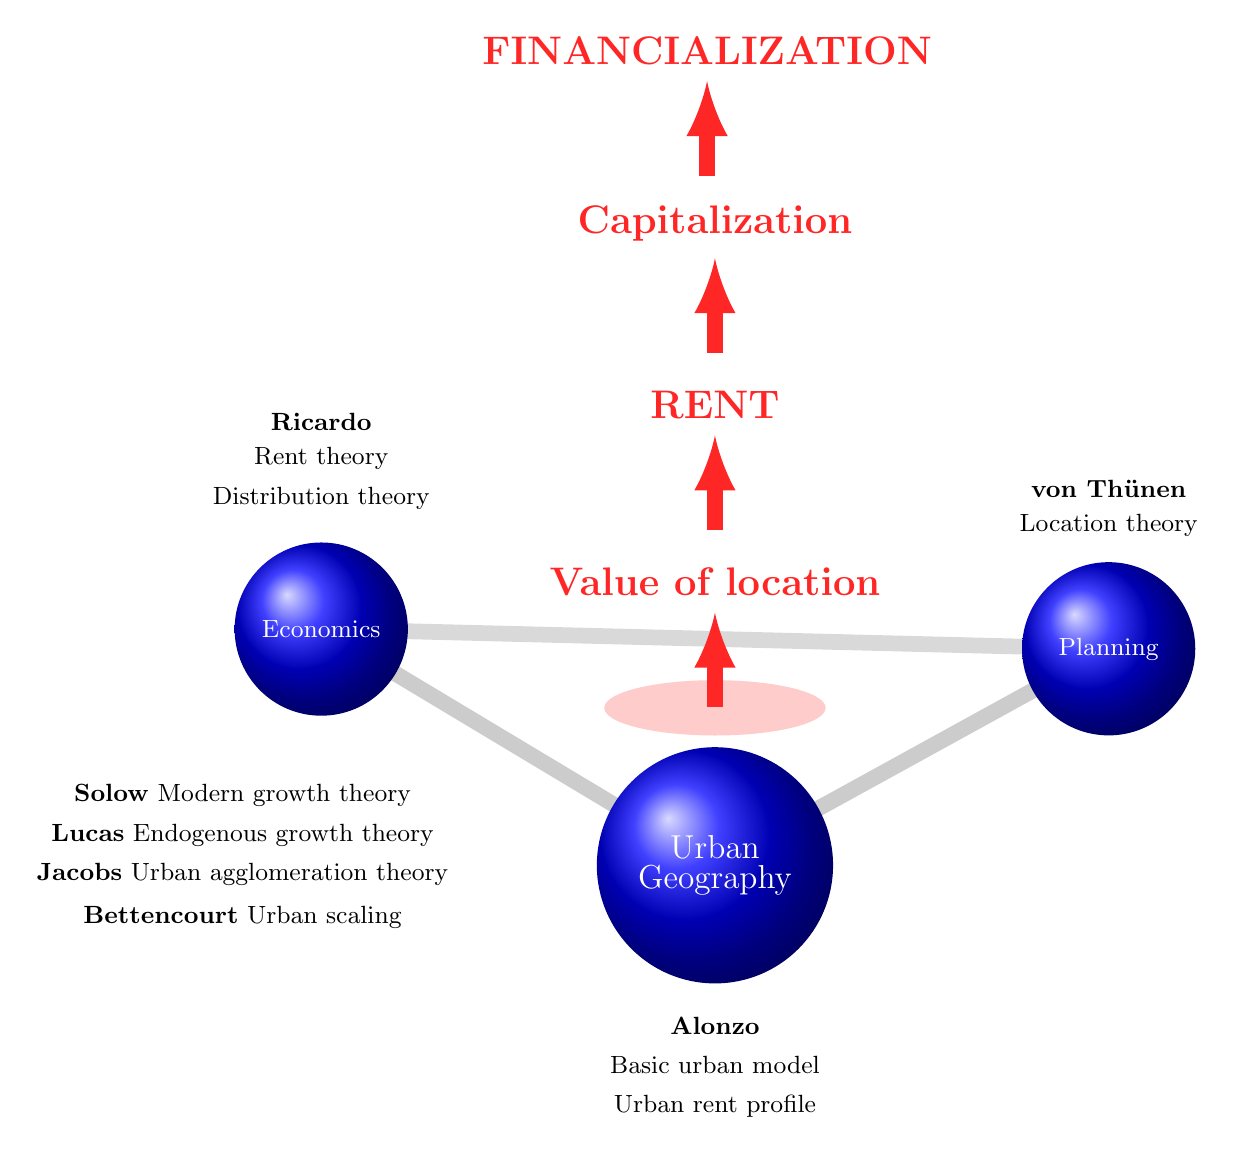
\begin{tikzpicture}{scale=.5}
% Find color for ball. Stop line short of node
\coordinate (planning) at (5,.75); % Preface
\coordinate (economics) at (-5,1); 
\coordinate (Ricardo) at (-5,1.4);
\coordinate (Solow) at (-6,1.25);
\coordinate (geography) at (0,-2); % History
\coordinate (finance) at (0,5); 

\draw [line width=2mm, black!15, ] (planning)--(economics);
\draw [line width=2mm, black!20, ] (geography)--(economics);
\draw [line width=2mm, black!20, ] (geography)--(planning);
%\draw [line width=2mm, black!25, ] (geography)--(finance);
%\draw [line width=2mm, black!20, ] (planning)--(finance);
%\draw [line width=2mm, black!20, ] (finance)--(economics);
%color=black!60!red
%\shade [ball color=blue!70] (5,5) circle (1.1cm)node[white] {\textbf{Planning}};
 
\node [circle,shading=ball,  minimum width=2.2cm, white, align=center] (ball) at (planning) {Planning};
\node [circle, shading=ball, minimum width=2.2cm, white, align=center] (ball) at (economics) {Economics};
\node [circle,shading=ball, minimum width=3cm, white, align=center] (ball) at (geography)[text width=2cm] {\large Urban \\ Geography};
%\node [circle, shading=ball, minimum width=2.4cm, white, align=center] (ball) at (finance)[text width=2cm] {Finance};
%\node at (-.3,-.1) [red] {\Large \textbf{RENT}};

\node at (planning) [above=1.8cm] {\textbf{von Th\"unen}};
\node at (planning) [above=1.3cm] {Location theory};

\node at (Ricardo) [above=2cm,]   {\textbf{Ricardo}};
\node at (Ricardo) [above=1.5cm] {Rent theory};
\node at (Ricardo) [above=1.0cm] {Distribution theory};

% \node at (Solow) [below=1.6cm, align=left] {\textbf{Solow:}};
\node at (Solow) [below=2.1cm, align=left] {\textbf{Solow} Modern growth theory};
\node at (Solow) [below=2.6cm, align=left] {\textbf{Lucas} Endogenous growth theory};
\node at (Solow) [below=3.1cm, align=left] {\textbf{Jacobs} Urban agglomeration theory};
\node at (Solow) [below=3.65cm, align=left] {\textbf{Bettencourt} Urban scaling};

\node at (geography) [below=1.8cm] {\textbf{Alonzo}};
\node at (geography) [below=2.3cm] {Basic urban model};
\node at (geography) [below=2.8cm] {Urban rent profile};
%\node [circle, shading=ball, minimum width=2.4cm, white, align=center] (ball) at (finance)[text width=2cm] {Finance};

\fill[red!20] (0,0) ellipse (40pt and 10pt);
%\node[red]at (1.2,0) {\large SPACE};
\begin{scope}[shift={(0,-.34)}]
\draw [line width=2mm, red!85, -latex ] (-.1, 7.1)--++(0,1.2)node[above=-.1] {\Large \textbf{FINANCIALIZATION}};
\draw [line width=2mm, red!85, -latex ] (0, 4.85)--++(0,1.2)node[above=-.1] {\Large \textbf{Capitalization}};
\draw [line width=2mm, red!85, -latex ] (0, 2.6)--++(0,1.2)node[above=-.1] {\Large \textbf{RENT}};
\draw [line width=2mm, red!85, -latex ] (0, .35)--++(0,1.2)node[above] {\Large \textbf{Value of location}};
%\draw [line width=2mm, red!85, -latex ] (0, -2)--++(0,-.8)node[above=-.1]  {\Large \textbf{SPACE}};
\end{scope}
\end{tikzpicture}
\caption[Linking space and urban rents to the effects of financialization.]{Space and urban rents play a foundational role in urban economics, geography, and planning. We extend the analysis of urban rents to model the effects of financialization.}
\label{fig-fields}
\end{figure}
In this thesis, to analyze the distribution of the value created in the city, we employ the idea of spatial rent, and put it into a model that allows for financialization of the urban housing market. This work therefore draws together insights from urban economics, geography, and planning. A central, shared concern in all three fields is geographic space: in all three, locational value gives rise to locational rents,\footnote{See Sprung-Keyser and Porter \cite{medina-olivaresJointModelLongitudinal2023} for a recent paper confirming that the is capitalized into land rents.}  explaining the dynamics of economic development, and the spatial distribution of human activities, respectively. 

The ultimate goal of this work is to develop a modern urban theory of rent, linking spatial rent, housing markets, and urban production. 
Figure~\ref{fig-fields} illustrated both the synthetic aspect of our analysis and the direction in which we develop existing work. The following sections introduce how this work fits in the literature and the basic structure of the core model, then list its main contributions, and give an outline for the thesis.

\subsection{Theoretical Background}

This thesis draws on work from several disparate traditions in order to model how the value created by cities is distributed.

To model the distribution of locational rents in an urban system, we need to go back to the classical theory of rent. The concept of economic rent was developed by the classical economists of the late eighteenth and early nineteenth centuries to explain how wealth was created and distributed in an agricultural society. David Ricardo \cite{ricardoEssayInfluenceLow1815} elaborated the classical theory of land rent and distribution in 1815.
Johann von Th\"unen \cite{vonthunenIsolirteStaatBeziehung1826} produced the first formal treatment of spatial economics and economic geography in 1826. Much later, in 1961, William Alonso (and others) \cite{alonsoModelUrbanLand1960} applied the Ricardian and von Th\"unen theory to the urban system, launching modern urban rent theory.  The spatial implications of the classical analysis were brought forward into modern urban theory, but the distributional implications were not. 

As Alonso and others were developing urban rent theory, Robert Solow \cite{solowContributionTheoryEconomic1956} developed modern growth theory, setting off a flood of work on economic growth that spilled into urban theory and connected with a rich body of work on economic development and the value created in cities, including work by Jacobs \cite{jacobsEconomyCities1969}, Lucas \cite{lucasMechanicsEconomicDevelopment1988}, Bettencourt \cite{bettencourtGrowthInnovationScaling2007}, and others. 


Our model therefore brings together three theoretical elements: an urban spatial model,  a model of the scaling of wealth in urban centers, and an income distribution model. %We incorporate that scaling result into the standard urban model, building of the work of William Alonso and others. 
We call the combined model 

To model the effects of financialization on wealth distribution, we combine their insights with a return to the classical focus on distribution.  Since an essential feature of cities is that they grow, we also draw on growth theory that looks at agglomeration effects and scaling laws to account for how distribution is affected by scale.  We also draw on neoclassical economic theory for its explanations of how the value of production in firms is shared among the owners of various resources.  Our work brings these traditions together into an integrated picture that allows us to look at wealth distribution within a spatial model that includes productivity and growth. 

What has been missing until now is a detailed account of who gets the land rents in the modern urban system. Our contribution is to extend the analysis of urban rents to take into account the effects of financialization, which is fundamentally a distributional process. This is a significant step because, while classical rent theory is the foundation for urban rent theory, the distributional aspects of the classical theory have not been applied. Meanwhile, standard models of financial operations are spaceless. This means the standard models don't relate them to spatial rents.\footnote{In describing any theory we need to identify the kinds of objects that are theorized. Financial analysis theorizes assets, debts, flows of revenue and costs, and the rates of change or exchange of these quantities over time. These are inherently spaceless because they are accounting entities, completely independent of location. It matters where a worker or a farm is. It does not matter where and dollar or a rouble is.} Our solution is to explicitly embed the normally spaceless analysis of investment decisions in a spatial model with locational rents.

The model makes it possible to analyze the potential macro effects of financial capital capturing spatial urban rents. Our focus is on changes in who captures these rents, and how that affects the productivity of the city. The distribution of locational rents, we believe, goes some distance to explaining core social issues like class structure, inequality, and political power.

\section{Modelling financialization of urban housing markets}
In order to develop an analysis of the distributional effects, we build a model with three components: an urban housing market, a financialization process, and an urban production system. The housing market sub-model distributes the ownership of the housing stock that comes up for sale in each period based on bids. % Both new entrants to the labour pool and financial investors can bid. If a new entrant fails to buy  housing that agent becomes a renter. 
The market determines the price for each unit. The price may depart from the market value of the services that each unit provides, providing the opportunity for speculative gains. Finally, the financial model determines the size of bids for investors based on the availability of capital and estimates of rental income and capital gains.

%the\cite{alonsoTheoryUrbanLand1960}, calling the combined sub-model the \gls{Alonso-Jacobs cycle} because there is a positive feedback between population size and wages. This feedback loop will be vulnerable if financialization extracts the new wealth generated by agglomeration effects, reducing wage growth and therefore the ability of the city to grow, because wage growth is what drives population growth and further agglomeration. The green boxes in the figure represent the theoretical justification of the primary simplifications in the model. 

\begin{figure}[!ht]
\centering
\includegraphics[scale=.60]{fig/flow-impacts.png}
\caption[The housing market component of the model.]{The housing market component. Financialization affects both the allocation of housing and its allocation of rents.}
\label{fig-impacts}
\end{figure}

Figure~\ref{fig-impacts} shows the logic  of the first component, the housing market model.
It shows two primary effects financialization has on the housing market: how it allocates
the housing stock, and how it allocates the \glspl{rent} generated by the urban system. 
The first effect of financialization, on housing allocation, arises because tenants replace owners. While owner-occupiers share in the growing land rents generated by urban agglomeration effects, tenants do not. As a result, a declining fraction of urban residents accumulate capital through their participation in the housing market, and therefore fewer enter the class of workers with both wage and capital income defined by John Roemer \cite{roemerGeneralTheoryExploitation1982}. 

The second effect of financialization on the market is in the allocation of spatial rents, generated in part by the growing productivity of cities. Rents generated by the \gls{agglomeration} economies in the urban system are diverted to largely non-resident owners, away from investment in local production or amenities, as tenants replace owner-occupiers.

\begin{figure}[!ht]
\centering
\includegraphics[scale=.70]{fig/flow-financialization.png}
\caption[The financialization component of the model.]{The financialization component. There is a feedback loop in which new investors drive up demand and thus drive up prices.}
\label{fig-financial-cycle}
\end{figure}

Figure~\ref{fig-financial-cycle} illustrates the second component of our model, the financialization process. We develop an explicit model of investor behaviour to explain the market decisions of buyers and the role of financial capital. The key observation is that investors enter the housing market. In doing so they drive up prices by increasing total demand. The rising price generates an expectation of capital gains, which enter the investors' calculations. Investors have, as research shows, better access to capital than most new entrants to the housing market. When the financial sector, the bank in the model, makes more capital available, the pattern of ownership shifts, as illustrated above.

Figure~\ref{fig-alonso-jacobs-cycle} illustrates the third component, the feedback between population and productivity. The green blocks represent the theory linking the relevant variables.  On the lower right, ``Scaling'' refers to the literature on agglomeration effects. On the upper right, neoclassical distribution theory provides a model linking productivity with wages.  On the left, the bid rent function links wages and population.


\begin{figure}[!ht]
\centering
\includegraphics[scale=.7]{fig/flow-alonso-jacobs-cycle.png}
\caption[Production system.]{The production system component, incorporating the urban scaling of wealth in the urban spatial model. We refer to this coupling of two difference equations  as the Alonso-Jacobs cycle.}
\label{fig-alonso-jacobs-cycle}
\end{figure}

A fundamental feature in recent empirical work on scaling laws is the persistent relationship between population and productivity. The productivity of cities increases superlinearly with population. Cities are the locus of a positive feedback loop with rising populations raising productivity, and rising productivity attracting more people and resources, a theoretical argument associated with the work of Jane Jacobs \cite{jacobsEconomyCities1969}, with strong empirical support from recent work on the scaling of urban productivity  \cite{bettencourtGrowthInnovationScaling2007, bettencourtOriginsScalingCities2013, dongUnderstandingMesoscopicScaling2020, loboUrbanScalingProduction2013}.


Combining these three components, we have an extended theory of urban rent built on a foundation of theory that goes back to the \gls{classical economics} around the beginning of the 19$^{th}$ century and incorporating modern growth theory and modern urban theory. 

The resulting model suggests two basic hypotheses:
\begin{enumerate}
    \item Financialization of the housing market will result in the tenantization of the urban middle class as financial capital acquires more of the housing stock. % vs decline of the urban middle class
    \item Financialization of the housing market will result in reduced growth of urban productivity as the flow of rents is diverted from real investment to the financial sector.
\end{enumerate} 
 
\section{Contributions}
The overall goal is to provide a theory of the relationship between financialization and urban productivity. The main contributions towards achieving this goal are:
\begin{enumerate}
    \item  Incorporating \gls{classical rent theory} into an \gls{agent-based} urban model. This requires modelling how \gls{Ricardian rent theory}, a theory of distribution based on an agricultural economy, applies in an economy driven by human capital \gls{agglomeration} effects within the urban system. 

    \item Allowing the creation and distribution of rents to influence urban growth, productivity and  population structure. This requires articulating the links between the wealth production of cities and how the urban system evolves.

    \item Incorporating current research on \gls{urban scaling} into the core spatial urban model.  This requires drawing on empirical work to formalise the scaling relationship, which embeds productivity in an urban model. 

    \item Constructing an urban \gls{agent-based model} that is consistent with {neoclassical growth theory}. We show how the neoclassical framework can be implemented in the agent-based framework, and make a case for the usefulness of the approach in linking urban rents and productivity. 

    \item Integrating \gls{financial capital} into a standard spatial model of the urban system, making an explicitly spatial model of the financial structures, which have traditionally been formalized in a spaceless way.
    
    \item Integrating financial capital into an \gls{overlapping generations} population model of the urban system and articulating the movement of financial capital though the urban land market. 
    
    \item Using an agent-based model to examine how financial markets impact urban \glspl{land market}, producing a formal simulation model that illustrates the process of housing financialization. 

    % \item Testing for \gls{hysteresis} resulting from the business cycle in the urban system and exploring the \gls{resilience} implication's of the core spatial economic model.

    \item Building a model that can be easily extended to explore a range of issues, and used to evaluate policy options. The model combines clear and explicit theoretical assumptions with careful and transparent implementation of the logic. We have taken care to allow for both theoretical and policy-relevant extensions in the simulation,  building a base model that aims to be as simple as something like Alonso's urban model \cite{alonsoLocationLandUse1964}, but simulates the relevant system features and can incorporate a range of intervention types. 
\end{enumerate}


\section{Document overview}
There are two parts in the dissertation. Part~\ref{part-background} gives the background and introduces the theoretical framework for the analysis, linking financialization with classical rent theory, neoclassical production theory, neoclassical growth theory, the scaling literature, and urban spatial models. 

\begin{enumerate}
    \item Chapter~\ref{chapter-financialization} discusses finacialization.

    \item Chapter~\ref{chapter-rent} reviews the literature on rent and introduces an an approach % doest hat fix it? develops an approach ***E  i FIND THIS PHRASING A  BIT AMBIGUOUS. ARE YOU DESCRIBING HOW YOU DEVELOPED THE APPROACH OR LAYING OUT THE APPROACH??? suited to the analysis for this work.

    \item Chapter~\ref{chapter-space} develops the urban model of space drawing on the basic Alonso model.

    \item Chapter~\ref{chapter-growth} introduces growth theory, showing how our model is directly connected with this broad collection of linked theories. 

    \item Finally, Chapter~\ref{chapter-tramsmission} discusses the potential feedback by which financialization, can affect the productivity of the urban system. %mechanisms for the transmission of the immediate effects of financialization to city productivity and growth.
\end{enumerate}
 
\noindent Part~\ref{part-model} describes the methodology, model, and results.

\begin{enumerate}
    \item Chapter~\ref{appendix-methodology} introduces the methodology for the approach. 

    \item Chapter~\ref{chapter-model} details the model of the illustrative agent-based model of the urban system. This model has three  parts: first, a production function, modelling how urban regions generate wealth,  second, a model of an urban housing market, and, finally, a financial sector that can participate in the market. 
% \end{enumerate}

% \noindent Part~\ref{part-analysis} develops the analysis, implications, and extensions for the base firm and housing market model.

% \begin{enumerate}
    \item Chapter~\ref{chapter-results} introduces the results, including the
    %\item Chapter~\ref{chapter-ownership} shows the 
    basic ownership result %.
    %\item Chapter~\ref{chapter-tramsmission} experiments  with the base model, and an extension to consider spillover productivity effects.
    % \item Chapter~\ref{chapter-extensions} introduces several extensions including amenity and transportation.
    % , and an extension to include amenity, respectively. 
    The experiments explore the static and dynamic effects of interventions in each case. % including our conclusions about the resilience of our social structure in the face of financialization.
    % \item \item Finally, Chapter~\ref{chapter-conclusions} draws conclusions from the work.
\end{enumerate}

\noindent Part~\ref{part-conclusions} %sketches future work and 
concludes. 

\begin{enumerate}
    \item Chapter~\ref{appendix-future-work} discusses future work. 
    \item Finally, Chapter~\ref{chapter-conclusions} draws conclusions from the work.
\end{enumerate}



% ADD BACK IN
% \begin{figure}
% \centering
%  \begin{tikzpicture}%[scale=.8]
    \tikzstyle{every node}=[font=\small]
%\draw[help lines,step=.5] (0,-11) grid (11,11);

\coordinate (aa) at (-1.5,7.5);%PREFACE
\coordinate (a) at (-1,10);%
 \coordinate (b) at (1.5,7); %history
\coordinate (c) at (6,10); %
\coordinate (d) at (9,9);%
\coordinate (ee) at (-4,7);%
  \coordinate (e) at (-1.5,5); %Community label
\coordinate (f) at (9.5,7.7); %???    PLAN
\coordinate (g) at (9,5); %Economics label
\coordinate (h) at (4.5,7);%tenure
\coordinate (ii) at (-4,4);%
   \coordinate (i) at (1,4);  
\coordinate (j) at (3,3.5);%whatis
\coordinate (k) at (6,4);%
 \coordinate (l) at (6.5,3.5);%joint
\coordinate (mm) at (-1.9,1);%coops
 \coordinate (m) at (1,1);%community grey circle
  \coordinate (n) at (3,1); %
  \coordinate (o) at (9.5,1); %efficiency
				 \coordinate (oo) at (6.5,1);%
				  \coordinate (o1) at (10.7,2);	 \coordinate (o2) at (10.7,0);%Propositions
\coordinate (p) at (9,-1.5);%externalities
				
\coordinate (qq) at (-4,-2);
\coordinate (q) at (-1,-1);%innovation
 \coordinate (r) at (3.2,1.2);%trans
  \coordinate (s) at (3.2,-1.2);%capital
 \coordinate (t) at (6.5,-2);%pubgoods
\coordinate (AA) at (-2,-5);%
 \coordinate (A) at (1,-5);%
\coordinate (B) at (3.7,-4); %
\coordinate (C) at (4.2,-4);%forestryEC
\coordinate (D) at (-1,3);%foresters
\coordinate (EE) at (-1,-8); \coordinate (E) at (1,-8); \coordinate (F) at (3,-8); \coordinate (G) at (6,-8); \coordinate (H) at (10,-4);%Policy
\coordinate (II) at (-4,-11);  \coordinate (I) at (1,-11); \coordinate (J) at (3,-11); \coordinate (K) at (6,-11); \coordinate (L) at (10,-11);
%\coordinate (M) at (coordinate); \coordinate (N) at (coordinate); \coordinate (O) at (coordinate); \coordinate (P) at (coordinate);
%\coordinate (Q) at (coordinate); \coordinate (R) at (coordinate); \coordinate (S) at (coordinate); \coordinate (T) at (coordinate);
% \fill[red, fill opacity=.8] (0,0) circle (4cm);
\fill [gray, fill opacity=0.2] (m) node [text width=2cm, black, opacity=1] 				(community)	{} circle (3cm);
\fill [gray, fill opacity=0.1] (oo)  node [text width=2cm, align=left, black, opacity=1] 		(econ) {} circle (3.5cm);
\node at (e) [ ] 		(comLtabel) {COMMUNITY};
\node at (g) [ ] 		(ecLabel) {ECONOMICS};
				%\draw (0,3.2,1) node [text width=1.5cm, text centered] {$Economics$};
			%\draw [fill=red, fill opacity=0.3]  (aa) node [ text width=2cm, black, opacity=1] 									(preface)		{PREFACE: Why, claims} circle (1.4cm);
\node [circle, draw,  fill=gray, opacity=.5,, text width=1.5cm] at			 (aa) 		(preface)		{PREFACE};
\node [] at			 (f) 		(plan)		{\Huge PLAN};
			%\draw [fill=blue, fill opacity=0.35] (b)node [text width=2cm, align=center, black, opacity=1] 			(history){History: New is Old} circle (1.2cm);
\node[circle, draw, text width=1cm, align=center, black, opacity=1]at 	(b)(history){History} ;
			%\draw [fill=pink, fill opacity=0.5] 		(h) node [text width=2cm, black, opacity=1] 								(tenure) 	{\color{black}tenure} circle (1.2cm);
\node[circle, draw,  text width=1cm, align=center, black] at 				(h) (tenure) 	{tenure} ;
\node[circle, draw,  text width=1.5cm, align=center]at							 (j) (whatis) 	{\color{black}What is Community Forestry} ;
\node[regular polygon, regular polygon sides=6, draw, align=center]at (l) (joint) 	{\color{black}Joint\\  products} ;


%\node[circle, draw,  text width=2cm, align=center]at (h) (tenure) 	{\color{black}tenure} ;

%\draw [fill=red, fill opacity=0.5] (j) node [text width=2cm, black, opacity=1] 												(whatis)		{What is Community Forestry}circle (1.4cm);
%\draw [fill=orange, fill opacity=0.5] 	(l) node [text width=2cm, black, text opacity=1] 	               		(joint)	{Joint products}											 circle (1.2cm);
%\draw [fill=green, fill opacity=0] (1,5)node [text width=2cm,red, opacity=1] {Policy and change} circle (1.4cm);
%\draw (q) node [text width=1.3cm, align=center, black, opacity=1] (small)	 {Innovation} circle (1.1cm);
\node[circle, draw,  text width=1.3cm, align=center] at							 (q) (small)	 {Innovation} ;

\draw 	(mm) node [text width=1.3cm, align=center, black, opacity=1] 	(coops) 	{Coops} circle (.8cm);
%\draw [fill=orange, fill opacity=0.5] 	(s) node [text width=2cm,  align=center, black, text opacity=1] (capital) {Human \\and social \\capital} circle (1.2cm);
\node[regular polygon, regular polygon sides=6, draw, align=center] at (s) (capital) {Human \\and social \\capital} ;
%\draw [fill=gray, fill opacity=0.5] 			(o) node [text width=2cm, black, text opacity=1] 						(efficiency)	{Efficiency} circle (1.2cm);
\node[regular polygon, regular polygon sides=6, draw, align=center] at (o) (efficiency)	{Efficiency};
\draw [fill=gray, fill opacity=0.75] (o1) node [text width=.3cm, white, text opacity=1] (	P1)  {P1} 		circle (.5cm);
\draw [fill=gray, fill opacity=0.75] (o2) node [text width=.3cm, white, text opacity=1] (P2) {P2} 			circle (.5cm);

%\draw [fill=orange, fill opacity=0.5] (p) node [text width=2cm, black, opacity=1]					(externalities)	 {externalities} 			circle (1.2cm);
%\draw [fill=orange, fill opacity=0.5] (t)node [text width=2cm, align=center, black, opacity=1] (pubgoods) {public goods} 		circle (1.4cm);
%\draw [fill=orange, fill opacity=0.5] (r) node [text width=2cm, black, opacity=1] 							(trans)	{transaction costs} 		circle (1.1cm);
\node[regular polygon, regular polygon sides=6, draw, align=center] at (p) (externalities)	 {extern\\-alities};
\node[regular polygon, regular polygon sides=6, draw, align=center] at (t) (pubgoods) {public\\ goods} ;
\node[regular polygon, regular polygon sides=6, draw, align=center] at (r) (trans)	{trans\\ -action\\ costs};



%\draw [fill=yellow, fill opacity=0.15] 	(C) node [text width=2cm, black, opacity=1] 							(forestryEC){forestry \\ economics} circle (1.4cm);
\node[regular polygon, regular polygon sides=6, draw, align=center, fill=gray!.25] at (C) (forestryEC){forestry \\ economics};
\draw [] 	(D) node [text width=1.1cm, black, opacity=1] 							(foresters)	{foresters} circle (.8cm);

  %%%%%JOINT PRODUCTS  AND TRANSACTION COSTS
%\draw [fill=orange, fill opacity=0.5] (G) node [text width=2cm, black, opacity=1] 								{efficiency} circle (1.4cm);
  %%%%%%%%%%%%%%%%%%%%  POLICY CHANGE
\draw [fill=gray, fill opacity=0.1] 		(H)    node [text width=2cm, align=center, opacity=1] 										{Policy and change} circle (1.4cm);
%ADDITIONAL TOPICS
%\draw (J) node [text width=6cm, text centered] {Economic Development };
%\draw ()--();

\draw [gray, line width=2mm,-> ](preface)--(whatis);
\draw  [darkgray, line width=1mm,<- ](history)--(whatis);
\draw  [black, line width=1mm,-> ](tenure)--(whatis);
\draw  [black, line width=1mm,-> ](history)--(tenure);

\draw [gray, line width=2mm,-> ](whatis)--(joint);
\draw [gray, line width=1mm,-> ](joint) to [bend right=25](efficiency);
\draw  [gray, line width=1mm,-> ] (joint) to [bend left=20](capital);
\draw [gray, line width=1mm,-> ](joint) to [bend right=20](externalities);
\draw [gray, line width=1mm,-> ](joint) to [bend left=25](trans);
\draw  [gray, line width=1mm,-> ](joint)->(pubgoods);
\draw  [gray, line width=.5mm,-> ](capital) to[bend left=25](small);
\draw  [gray, line width=.5mm,-> ,dashed](joint) to[bend left=7](forestryEC);
\end{tikzpicture} 
% \caption{Document overview.}
% \label{fig-community-forestry}
% \end{figure}